
\subsection{CIVIS Back-end as a JS Runtime Environment}

The YouPower back-end is developed using the \textit{Node.js}\footnote{\url{https://nodejs.org/}} platform, a well-known JS based open source runtime environment for server-side applications. 
The platform is easily extensible and has a repository of libraries that support fast web development. 
% 
TU Delft prepared a virtual machine for CIVIS to host the WP3 back-end\footnote{\url{http://civis.tbm.tudelft.nl}}
using \textit{Nginx}\footnote{\url{https://nginx.org/en/}}, an http and reservse proxy server. 
% 
A \textit{Comodo}\footnote{\url{https://ssl.comodo.com/}} SSL certificate is installed on the server to provide secure communication (i.e. https). 

\textit{MongoDB}\footnote{\url{https://mongodb.org/}} is used as the WP3 back-end database. It is document-oriented, and has flexible data schema and expressive query language. 
A list of the data models at the back-end can be found at {\footnotesize\url{https://github.com/CIVIS-project/YouPower/tree/master/backend/models}}. 
Figure~\ref{fig:datamodel} shows the data model schema.
%
\begin{figure}
\centering
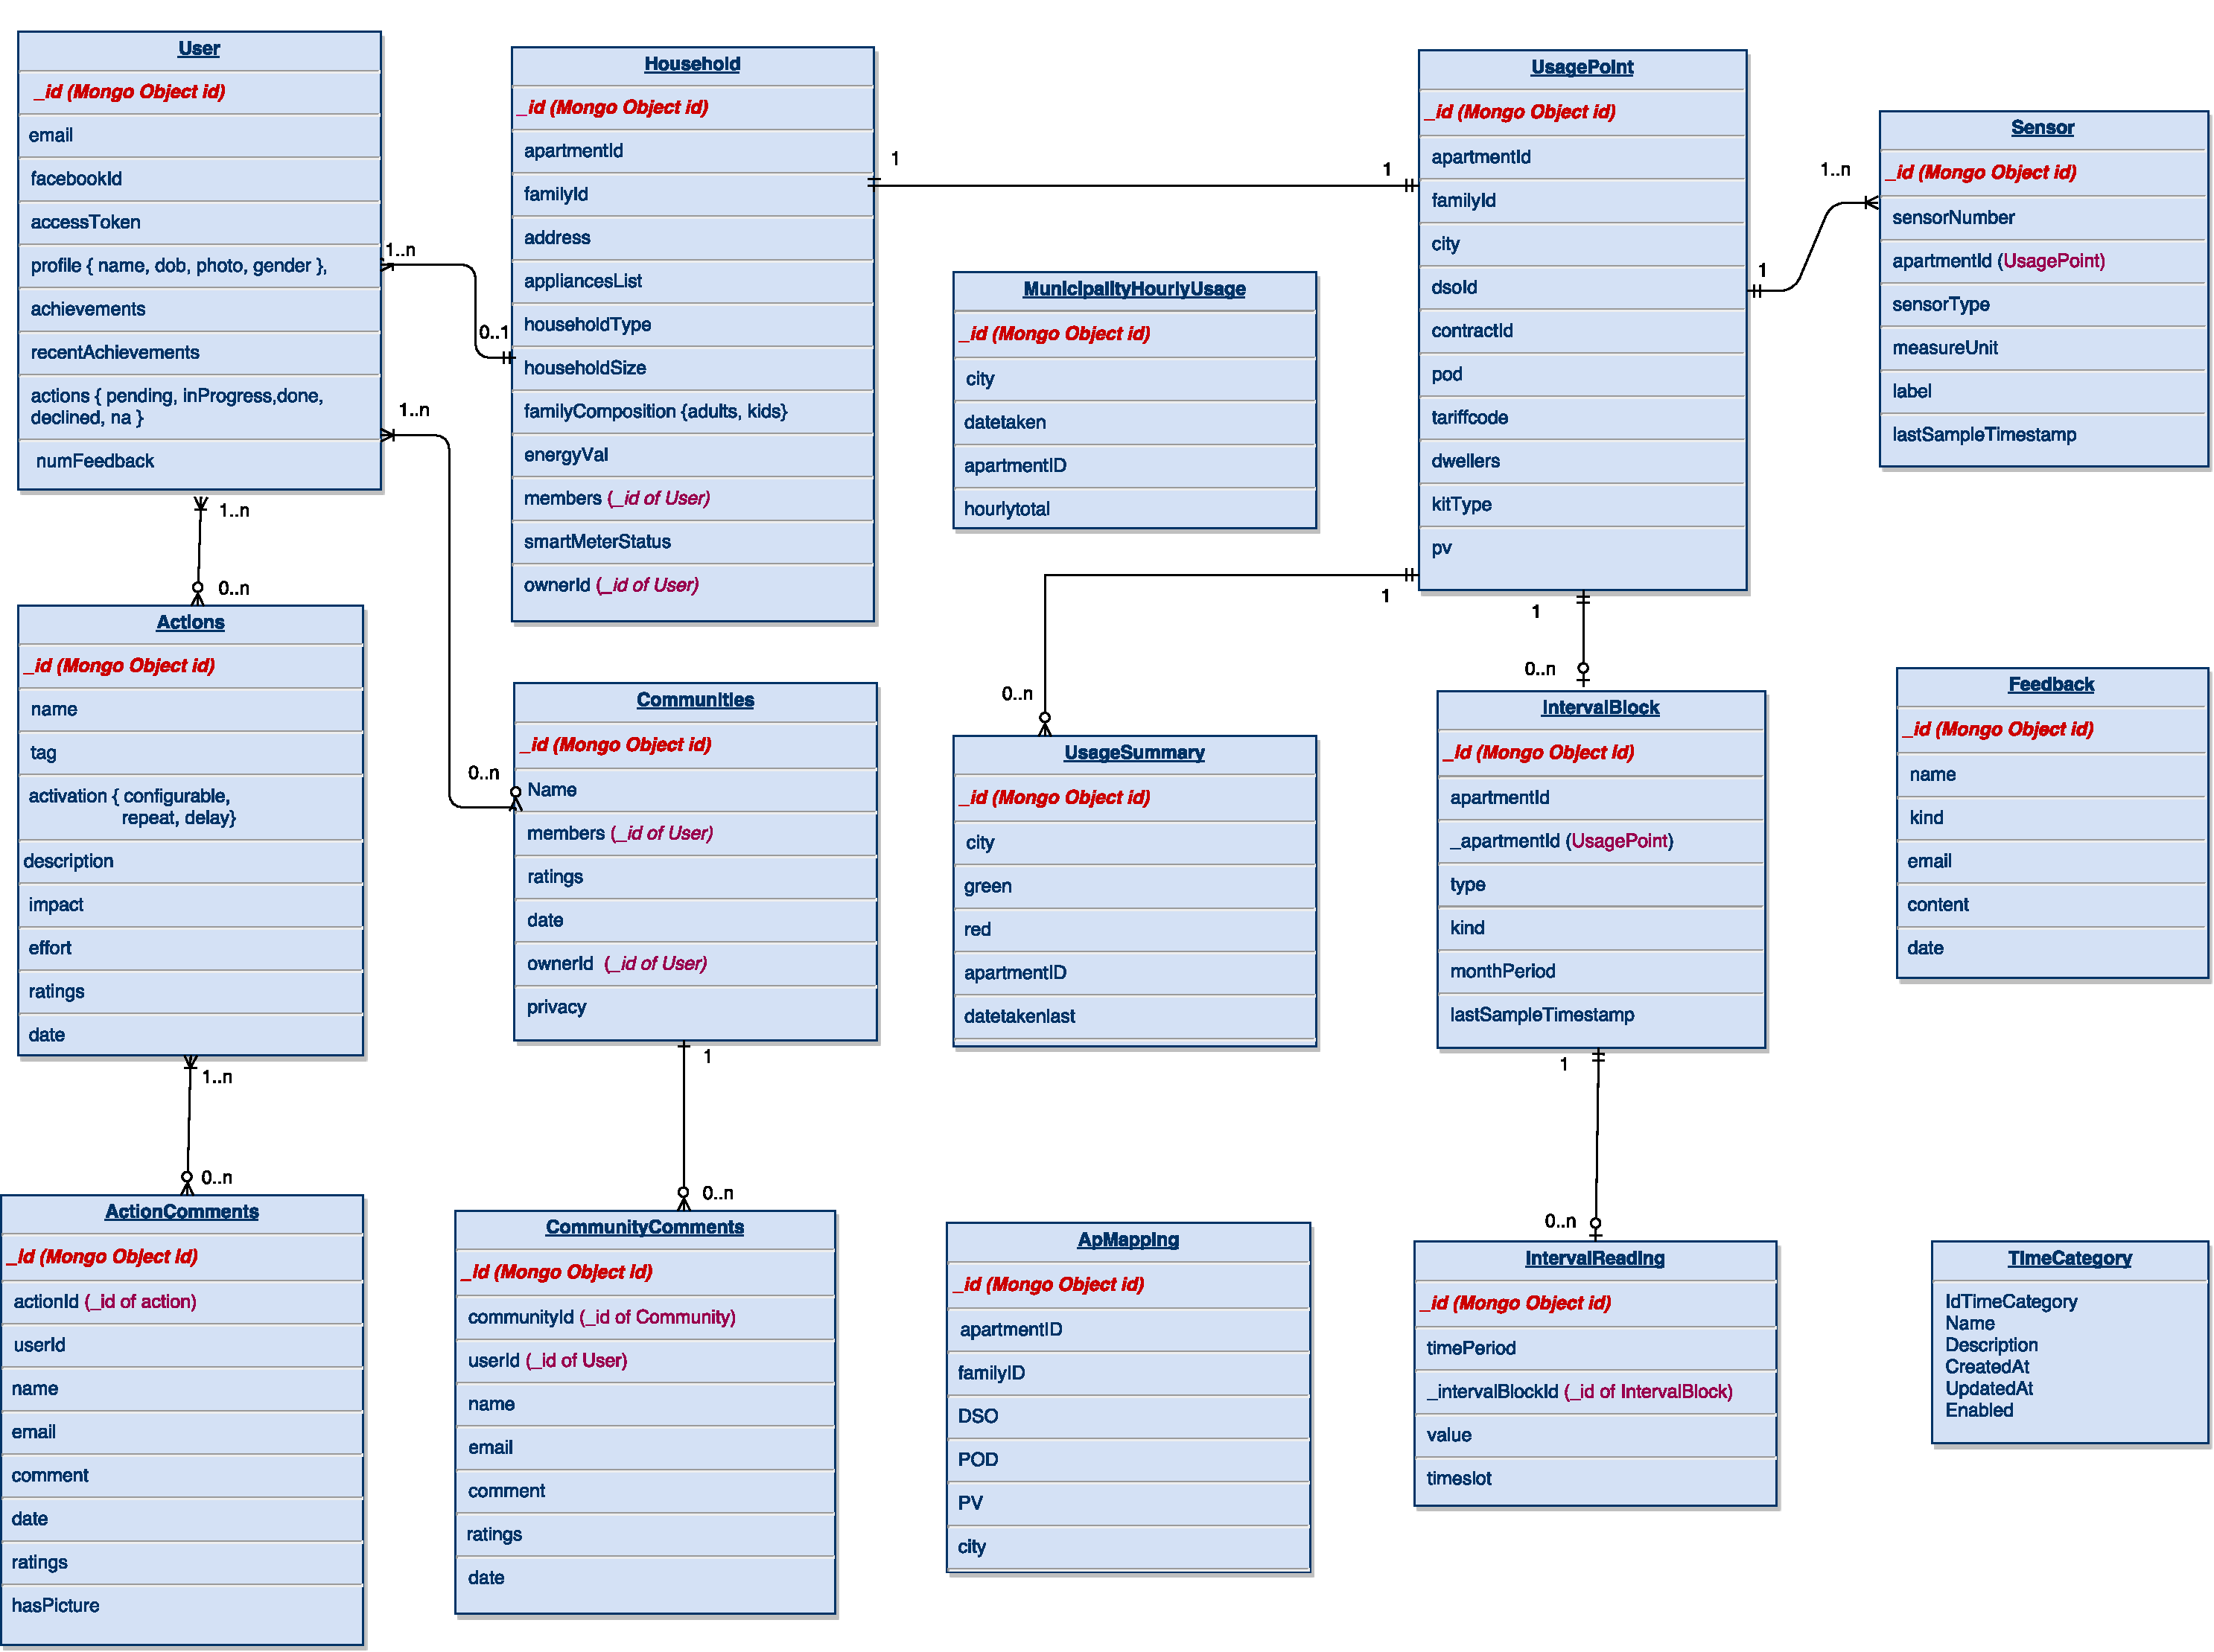
\includegraphics[height=.92\linewidth,angle=90]{img/7sdatamodel}
\caption{YouPower back-end data model schema}
\label{fig:datamodel}
\end{figure} 
% 

The noteworthy Node.js libraries used for the WP3 back-end development are as follows:

\begin{itemize}

\item Async.js\footnote{\url{https://github.com/caolan/async}}, which makes managing and combining asynchronous tasks easier. 

\item Express.js\footnote{\url{http://expressjs.com/}}, a Node.js application server framework we use as a basis for the REST API. 

\item Mocha\footnote{\url{https://mochajs.org/}}, a JavaScript unit test framework. 

\item Mongoose\footnote{\url{http://mongoosejs.com/}}, a MongoDB driver for Node.js. It provides a schema-based solution to model data. 

\item Passport.js\footnote{\url{http://passportjs.org/}}, for handling authentication of REST API requests for Node.js, both local (username password) and Facebook. 

\item Underscore.js\footnote{\url{http://underscorejs.org/}}, a JS library that provides over 100 utility functions. 
%\item Ionic Push\footnote{\url{https://apps.ionic.io/landing/push}}, for sending dynamic push notifications. 

\item Nodemailer\footnote{\url{https://nodemailer.com/}}, sending emails with Node.js.

\item Email-templates\footnote{\url{https://www.npmjs.com/package/email-templates}}, a Node.js module for rendering beautiful emails.

\item Fb\footnote{\url{https://www.npmjs.com/package/fb}}, a Node.js library for Facebook.

\item Moment.js\footnote{\url{http://momentjs.com/}}, a JS library to parse, validate, manipulate and display dates. 

\item APIDOC script\footnote{\url{http://apidocjs.com/}}, for inline documentation for the REST API. 

\item Node-xml2js\footnote{\url{https://github.com/Leonidas-from-XIV/node-xml2js}}, a simple XML to JavaScript object converter. 

\item Dateformat\footnote{\url{https://www.npmjs.com/package/dateformat}}, for formatting dates to custom formats. 

\item HTTPS\footnote{\url{https://nodejs.org/api/https.html}}, A nodeJs module used to make service calls over TLS/SSL. 

\item Querystring\footnote{\url{https://www.npmjs.com/package/querystring}}, for deserializing querystring to an object. 

\item Fs\footnote{\url{https://www.npmjs.com/package/querystring}}, for manipulating file in NodeJS. 
\end{itemize}

% 
The WP3 back-end interacts with the WP4 back-end, from which the former fetches relevant energy data that is particularly relevant for visualization of energy consumption/production and energy consumption signal. The availability of such data through the WP4 platform represents therefore a pre-condition for the ability of the app to correctly visualize such information. The WP3 back-end REST API documentation can be found at {\footnotesize\url{http://civis.tbm.tudelft.nl/apidoc/}}. 
% 

